\chapter{Introduction}
%\addcontentsline{toc}{chapter}{Introduction}
%

\selectlanguage{english}

%
Modern society faces a wide range of challenges that require complex and multifaceted solutions. The challenges posed by climate change and the necessity for clean energy in order to reduce greenhouse gas emissions intersect with the goals of economic growth and the global exchange of information, goods and people. Unprecedented issues are emerging from this increasingly technologically advanced and interconnected civilization. 

This PhD work was initiated amidst the most impactful public health crisis of our time, the COVID-19 pandemic. Despite all the negative facets of this pandemic, it unexpectedly gave a boost to a specific market : the emerging technology of deep ultraviolet violet light-emitting diodes (UVC LEDs), and the market is predicted to grow five-fold.\cite{Yole} Indeed the deep UV light, \textit{i.e.} with wavelengths ranging from 100 to 280 nm, has been demonstrated to inactivate the coronavirus accountable for the disease, thus making it harmless.\cite{GERCHMAN2020112044} Besides surface disinfection, UVC LEDs have many applications in water and air depolution, agriculture, printing and more.\cite{hsu2021perspectives} The material studied in this thesis, hexagonal Boron Nitride, is a candidate of choice for the elaboration of UVC LEDs due to its bright light emission in the deep ultraviolet.

This is a recent example of how technological innovations resulting from scientific research in materials science can provide a means to address the challenges of modern society. The European Union supports such research, in particular through the Flagship projects, which are large-scale research initiatives with an emphasis on technology transfer to industry. Three out of the four Flagship projects are closely related to materials science: Batteries30+ for the development of efficient and compact energy storage,\cite{batteries_flagship} Quantum Technologies\cite{quantum_flagship} for the quantum computers and algorithms and Graphene,\cite{graphene_flagship} which focuses on two-dimensional materials. All of these are research projects that could provide means to produce clean energy and store it. In all of these scientific areas, theory and numerical simulations are essential to support the experimental discovery of materials and guide the engineering of new devices. This is particularly relevant in Condensed Matter Physics which is the subject of this thesis. Since the discovery of Graphene and its extraordinary properties by Novoselov and Geim in 2004,\cite{novoselov2004electric} the two-dimensional materials such as Graphene, black Phosphorus, transition metal dicalchogenides (TMDs) and \acrfull{hBN} have attracted a great deal of attention. Indeed, they exhibit a range of electronic and optical properties that allow the design of devices for different applications, especially when different layers are stacked to form the so-called van der Waals heterostructures.\cite{geim2013van} The resulting devices are then very compact and fit very well into the technological trend of device miniaturization.

With the variety of optical and electronic properties offered by all the existing monolayers, and the ability to engineer them with factors such as stacking of different layers,\cite{sponza2018direct} twisting angle between them,\cite{latil2023structural, impellizzeri2022electronic} and straining\cite{blundo2021strain} as well as their interaction with substrates, the possibilities for devices are almost limitless. In this ecosystem, hexagonal Boron Nitride is a candidate of choice for its structural, electronic and optical properties.

% 


\section*{The process of luminescence}
Optical measurements are an efficient way to characterize materials and reveal the microscopic, quantum, interplay between electronic wavefunctions and electromagnetic field of light, and collective quantum effects in the crystal.\cite{dressel2002electrodynamics} In particular, spontaneous emission of light after an excitation, known as \textit{luminescence}, is the key property for the elaboration of light-emitting diodes.\cite{pelant2012luminescence}

For spontaneous light emission to happen in a semiconductor or insulator, there needs to be a population of excited electrons in the conduction band. The excitation can have different forms. It can be done with the electromagnetic field of external light, then the process is called photoluminescence. If the electrons are excited by an external beam of electrons colliding with the crystal, it is called cathodoluminescence. If they are excited by an external electric field, it is called electroluminescence, \textit{et cetera}. When the electrons are promoted to the higher-energy conduction bands, they leave an empty state in the valence band. This empty state can be thought of as a \textit{hole} in the Fermi sea of the valence states. It propagates with the opposite of the electron's momentum and has a negative effective mass. For light to be emitted, the excited electrons need to de-excite and go back to the empty states. We speak of radiative recombination of an electron-hole pair. When the hole and the electron have the same momentum (and the same spin and symmetry) the radiative recombination can happen because the emitted light carries an almost null momentum, hence respecting momentum conservation. The energy difference between the electron and the hole corresponds to the frequency of emitted light, multiplied by $\hbar$. 
However when the bottom of the conduction band is not at the same momentum than the top of the valence band, the light emission cannot happen directly because of momentum conservation. There needs to be a second-order process to exchange momentum. For instance, the excited electron can transfer its momentum to another one in the conduction band and then recombine with the hole. This process is known as Auger-Meitner recombination.\cite{delaney2009auger} Otherwise, the momentum exchange can come from the absorption or emission of a phonon, hence gaining or losing energy and momentum and finally leading to a radiative recombination. This is known as a phonon-assisted transition and it is the process that is studied in this thesis. 

Luminescence is often thought of as the reverse process of light absorption. Indeed in absorption, light with a frequency higher than the gap can excite electrons and promote them to the conduction band, with almost zero transfer of momentum. In the case of phonon-assisted transitions, the electron can be promoted to the conduction band at another momentum, thanks to the absorption or emission of a phonon. 

Because of this similarity, the spectra of absorption and of luminescence are quasi symmetrical for direct transitions. The slight asymmetry come from the phonon broadening of the electron density of states, known as the Stokes shift. However when considering phonon-assisted transitions, the asymmetry will be more pronounced because the interplay between direct and indirect processes will lead to quite different features in the two spectra.

In this thesis, we study the properties of different forms of \acrshort{hBN} and develop theoretical and numerical methods with the aim of reproducing and predicting their luminescence spectra from \textit{ab initio} calculations.


\section*{The peculiar properties of hexagonal Boron Nitride}
The first reported synthesis of Boron Nitride dates back from 1842.\cite{balmain1842xlvi} It is now available commercially under the form of a white powder and finds applications as lubricant or for its high thermal resistivity. It can be found under the form of a layered material composed of atomically thin layers arranged in a honeycomb lattice. High-purity crystals are synthesized under high-pressure and high-temperature conditions.\cite{watanabe2004direct} 
Different stacking of the layers lead to different stable or metastable polytypes. In this thesis we will be mainly concerned with the AA' and the AB stackings, that are illustrated in Fig. \ref{fig:hBN_stackings}. We will refer to the AA' polytype as hBN and to the AB polytype (or Bernal phase) as bBN. The atoms within a layer are bond by hybrid $sp^2$ bonds, while the interlayer interactions are of van der Waals type.
\begin{figure}[h!t]%
	\vspace{0.2cm}
	\setcapindent{2em}
	\centering
    \subfloat[AA' stacking]{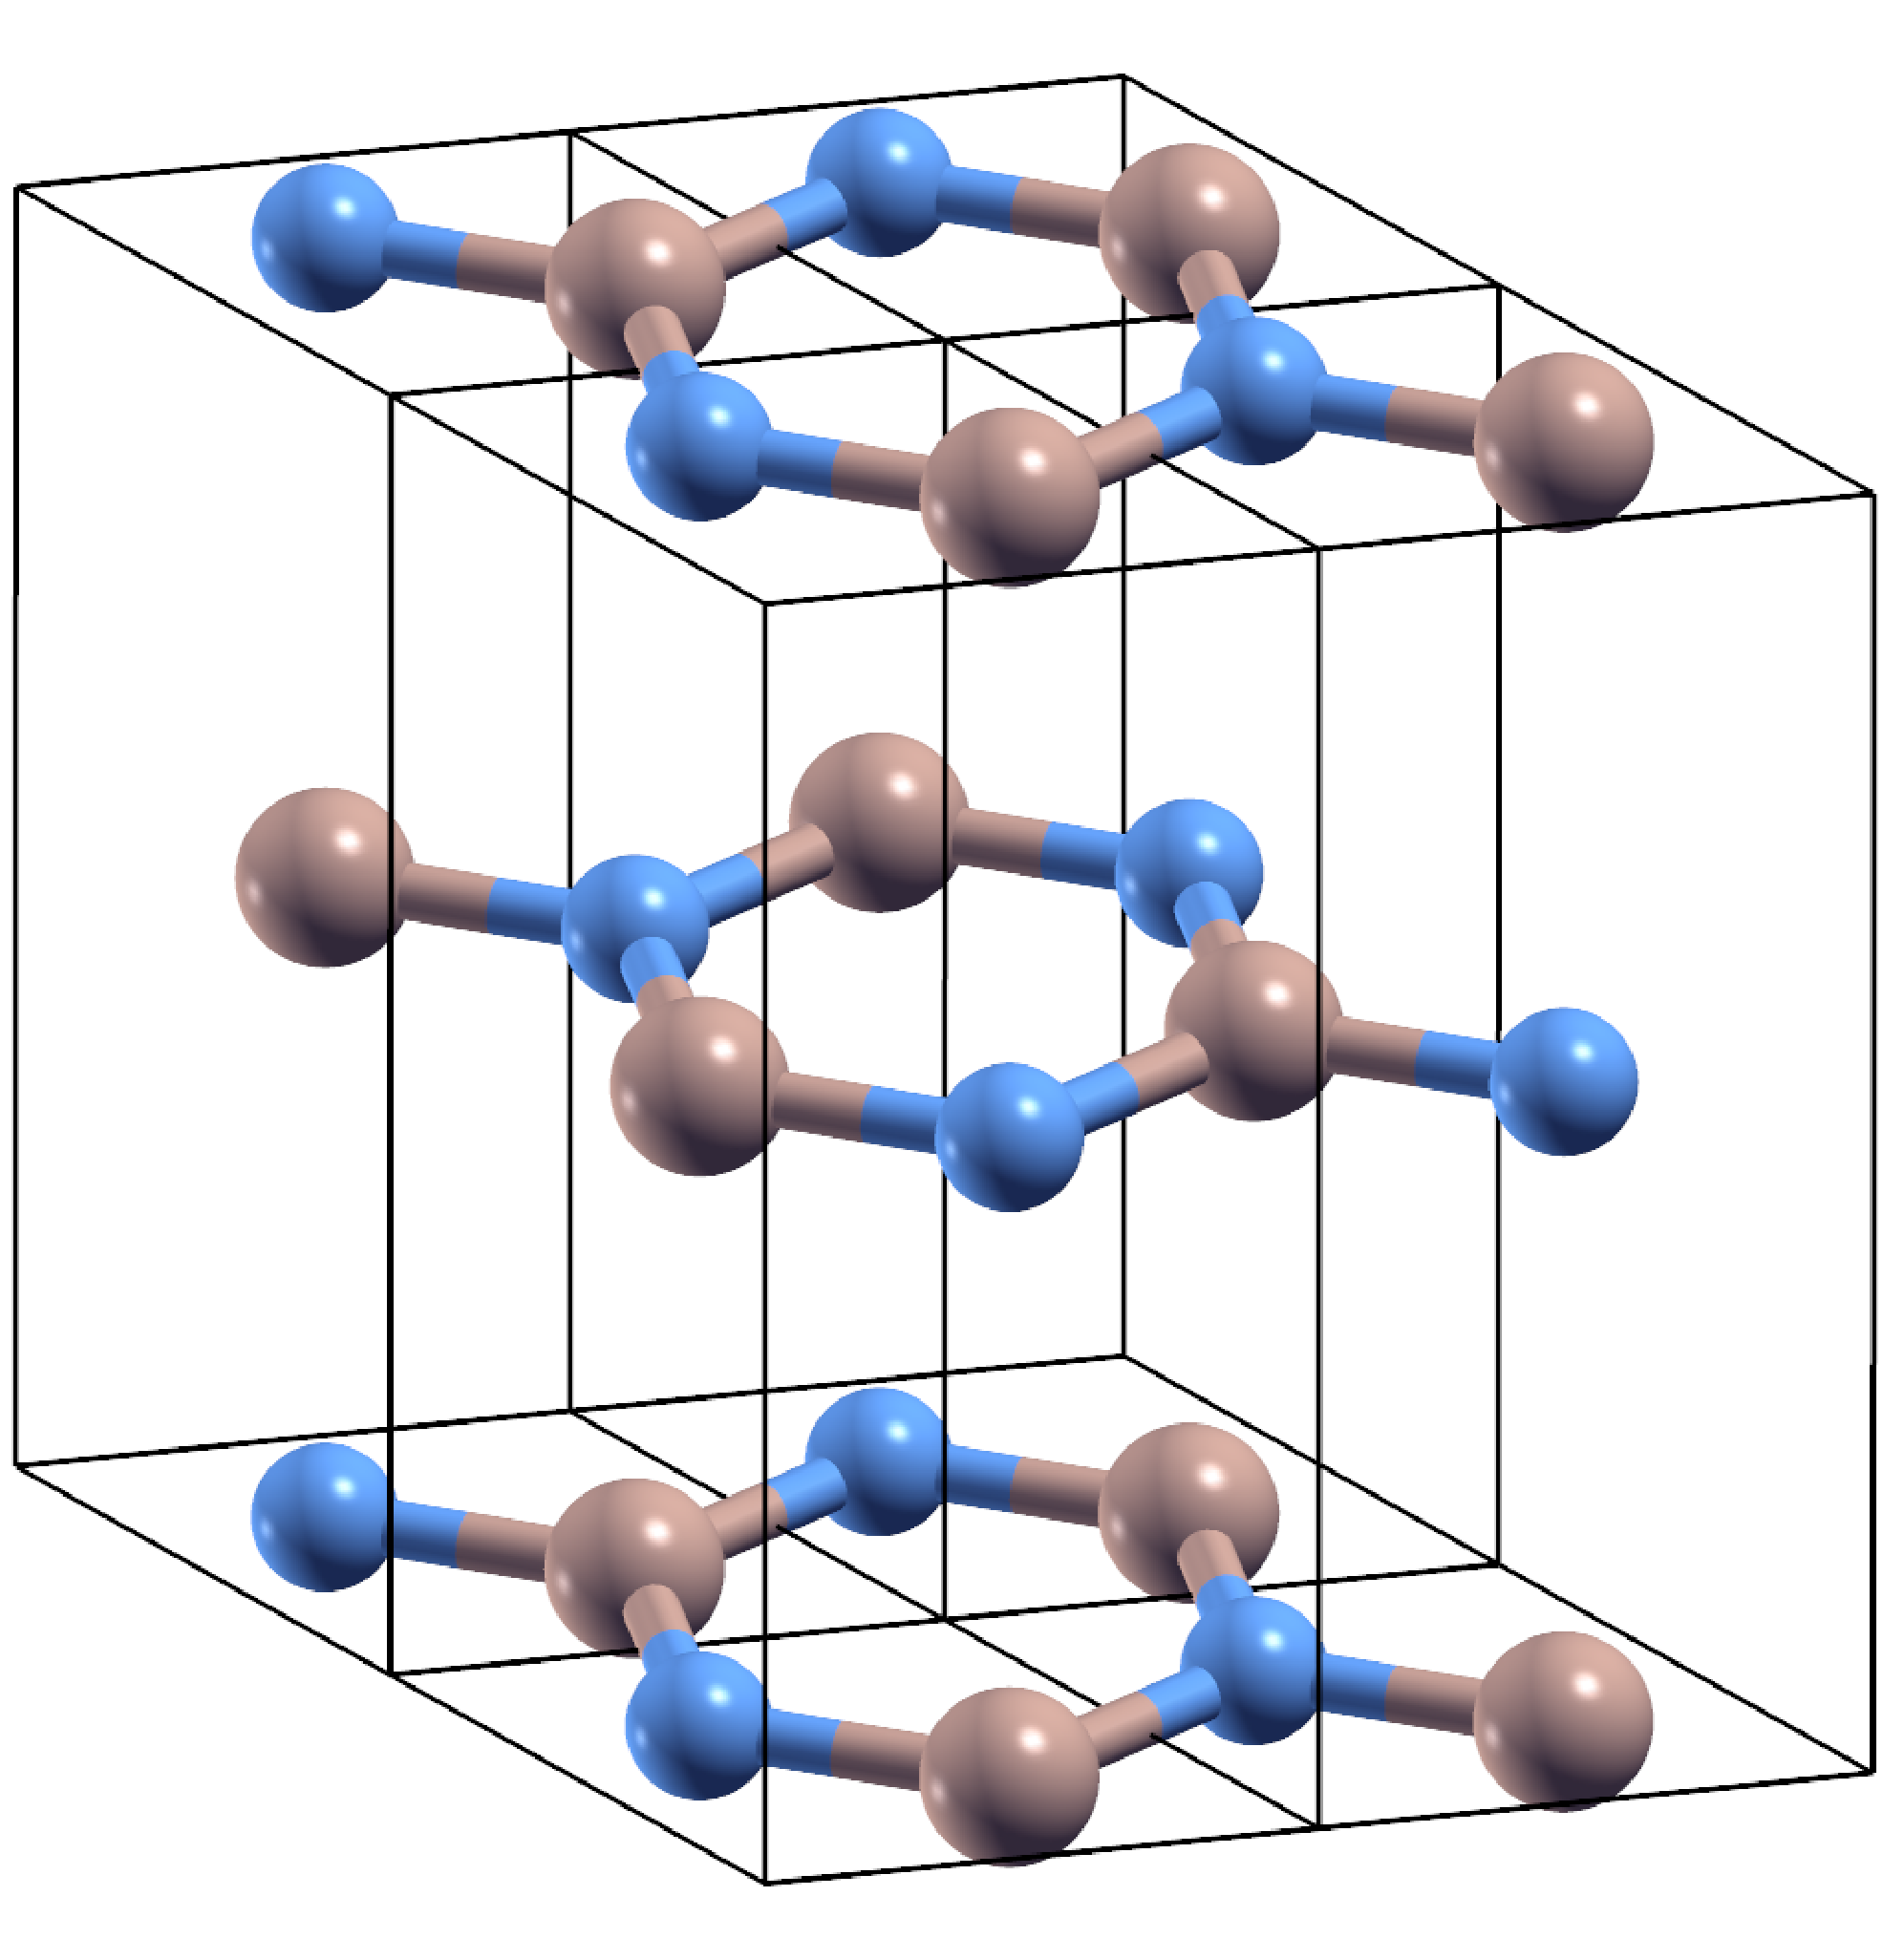
\includegraphics[width=0.42\textwidth]{intro/hBN_struc_crop.pdf}} \qquad
    \subfloat[AB stacking]{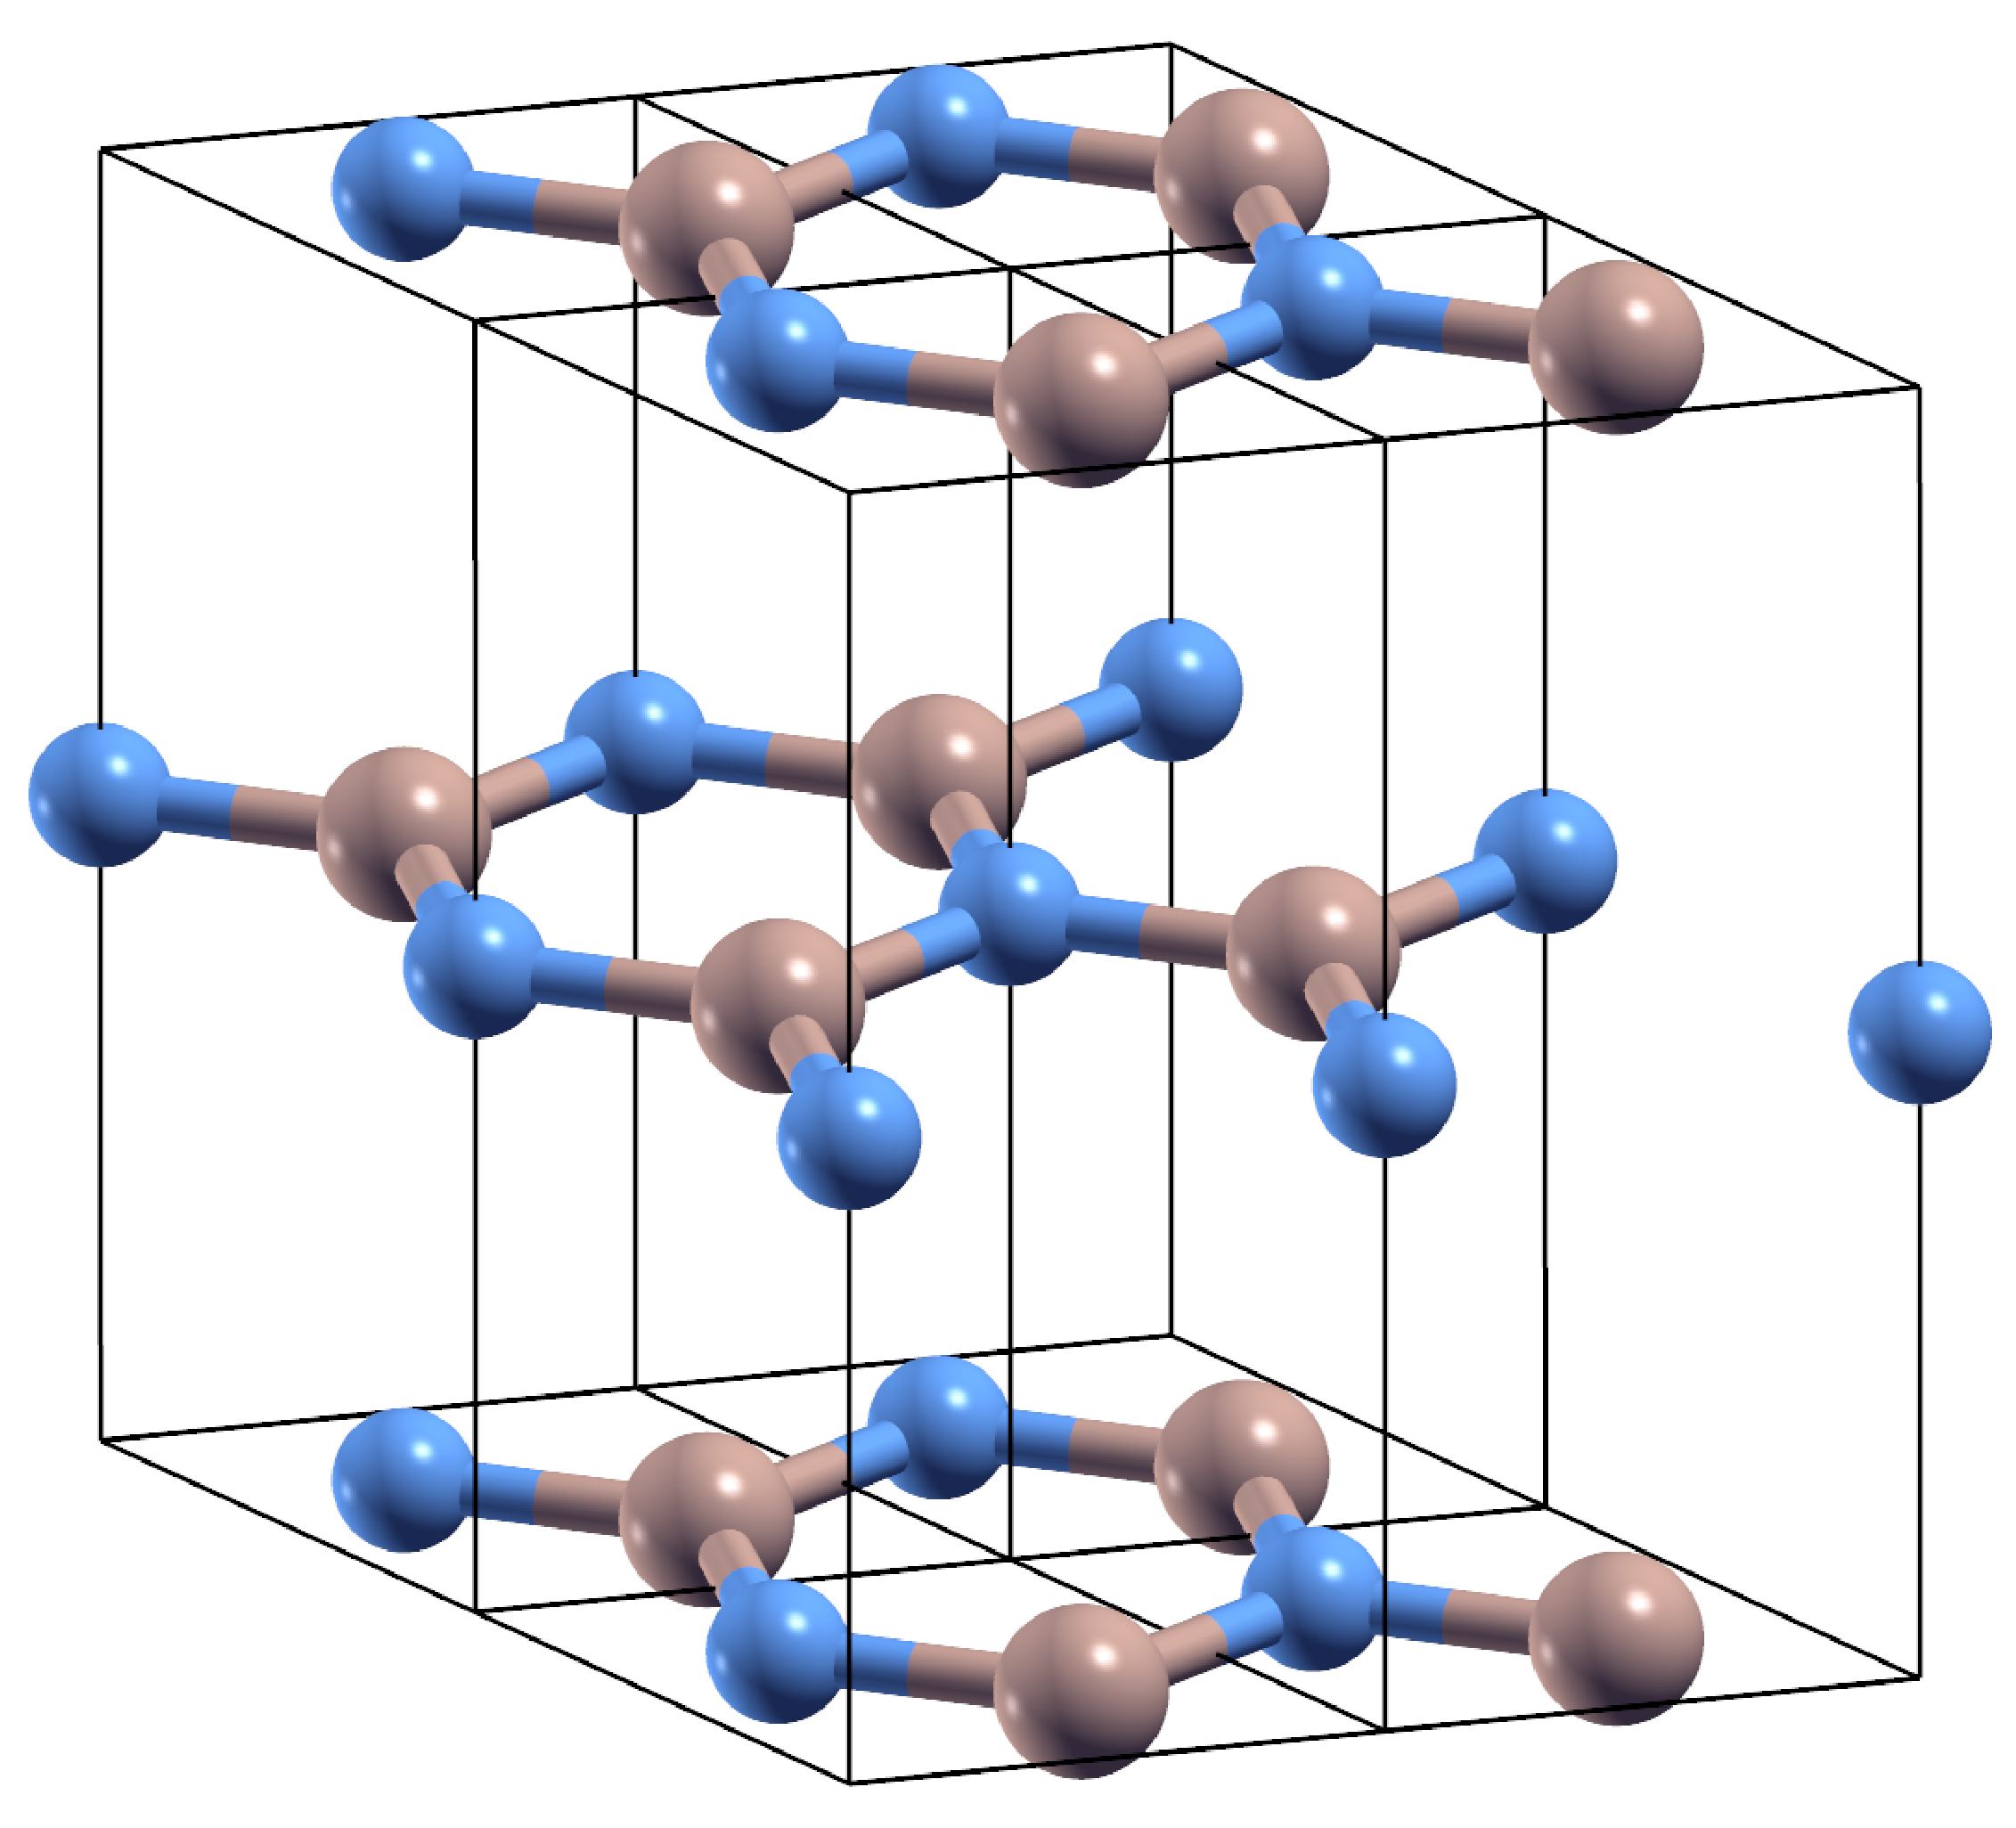
\includegraphics[width=0.45\textwidth]{intro/bBN_struc_crop.pdf}}%
    \caption{Two polytypes of hexagonal Boron Nitride where four hexagonal unit cells are shown. Boron atoms are represented with brown spheres, Nitrogen with blue ones. We will refer to the AA' polytype as hBN and to the AB polytype (or Bernal phase) as bBN.}
	\label{fig:hBN_stackings}
\end{figure}
%
hBN is stable at ambient pressure and room temperature. It is an insulator with a gap of about 6 eV. Due to its low lattice mismatch with Graphene and its insulating character, it is a substrate of choice and a good encapsulation layer for Graphene-based applications.\cite{kretinin2014electronic} It also has a variety of defect-related physics that can find applications for quantum computing,\cite{ivady2020ab} single photon emission\cite{grosso2017tunable} or bright color center emission.\cite{wigger2019phonon} However the property of interest for this thesis is the bright light emission in the deep UV domain and the rich features appearing in the luminescence spectra. hBN was shown to have a very high internal quantum yield, comparable to that of a direct gap material such as Zinc Oxide.\cite{schue2019bright} This is due to the strong exciton-phonon coupling enhanced by the anisotropy of this layered material and to the large density of transitions due to flat bands in the electronic dispersion.\cite{elias2021flat} Experimental luminescence spectra for the bulk material are abundant in literature, see for instance Refs. \cite{schue2019bright,cassabois2016hexagonal}. These spectra exhibit a fine structure due to the scattering with different phonon modes as was reproduced by first-principle calculations in Refs. \cite{cannuccia2019theory,paleari2019exciton}
However, obtaining the optical absorption spectrum experimentally requires more advanced equipment because \acrshort{hBN} absorbs in the \acrshort{UV} range. In Ref. \cite{artus2021ellipsometry} it was obtained using synchrotron radiation for a large range of frequencies. 
In general the absorption (or a quantity proportional to it such as the photoluminescence excitation\footnote{Photoluminescence excitation (PLE) is the measure of the luminescence intensity as a function of the energy of the laser that excites the system. The PLE signal is the highest where the system absorbs the most light.}) and the luminescence spectra have a strong asymmetry, as can be seen in Fig. \ref{fig:cl_ple}, because the state dominating the absorption is different from the one dominating the luminescence, which is at lower energy. Moreover the coupling with different phonon modes gives rise to multiple peaks in the luminescence spectrum, only visible in absorption with a very fine resolution because the direct peak overlaps with them. This will be explained in details in the body of this thesis.
\begin{figure}[h!b]
	\vspace{0.2cm}
	\setcapindent{2em}
	\centering
	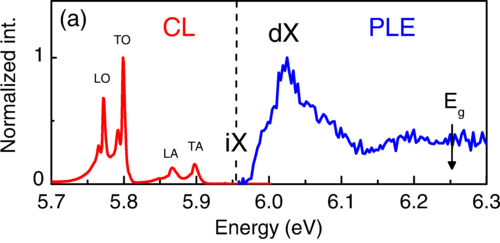
\includegraphics[width=0.9\textwidth]{intro/schue_cl_ple_crop.png}
	\caption{Comparison between the cathodoluminescence (red) and the photoluminescence excitation (blue), which is proportional to absorption of bulk hBN. iX and dX refer to indirect and direct exciton energy, respectively. $E_g$ indicates the gap energy.  Extracted from Ref. \cite{schue2019bright}.}
	\label{fig:cl_ple}
\end{figure}

As for the Bernal phase (\acrshort{bBN}), it was recently synthesized and characterized with optical measurements. Its photoluminescence spectrum was reported in Refs. \cite{rousseau2022bernal,rousseau2022phonon}. It seems to exhibit direct and indirect gaps very close in energy, as theoretically predicted in Ref.\cite{sponza2018direct}, giving rise to direct peak and phonon satellites with comparable intensities. This case is addressed at the end of Chapter \ref{chap:mBN}.

% @article{kim2013stacking,
%   title={Stacking order dependent second harmonic generation and topological defects in h-BN bilayers},
%   author={Kim, Cheol-Joo and Brown, Lola and Graham, Matt W and Hovden, Robert and Havener, Robin W and McEuen, Paul L and Muller, David A and Park, Jiwoong},
%   journal={Nano letters},
%   volume={13},
%   number={11},
%   pages={5660--5665},
%   year={2013},
%   publisher={ACS Publications}
% }

For a single layer, measuring the luminescence intensity is much harder because the signal is faint due to the low thickness of the material. To have a good resolution, one needs to be at cryogenic temperature in ultra-high vacuum, and have an extremely pure sample.
Cathodoluminescence measurements were performed for sheet thicknesses down to six layers,\cite{schue2016dimensionality} but the signal-to-noise ratio becomes too low for smaller thicknesses.\footnote{We mention for exhaustiveness Ref. \cite{shima2023cathodoluminescence} where cathodoluminescence was reported for a single layer of BN, however the signal-to-noise ratio is very small and this article has not been peer-reviewed yet.}
Photoluminescence measurements are equally difficult to obtain, but some results were published recently for monolayers grown by epitaxy on a Graphite substrate,\cite{elias2019direct,wang2022scalable} or mechanically exfoliated and deposited on an SiO$_2$ substrate.\cite{rousseau2021monolayer} These three spectra exhibit features that are quite different, and their interpretation is not unanimous. We address this question in Chapter \ref{chap:mBN}. 

On the theoretical point of view, absorption spectra are relatively easy to obtain from state-of-the-art \textit{ab initio} calculation, but luminescence is more difficult since it is an out-of-equilibrium process. Moreover, a general formulation of luminescence that includes both direct and phonon-assisted transitions on the same footing from first-principles is still lacking. This thesis contributes towards this goal.


% keep this for defense
% show electronic bands : hig gap, pDOS of valence at K is mostly Nitrogen, $\pi$ orbital(overlap of $p_z$, bonding)  . pDOS of conduction at M is mostly Boron, $\pi^*$ orbital \cite{galvani2016excitons,sponza2018direct}(overlap of $p_z$ with opposite coefficient, antibonding)\\



% @article{gorbachev2011hunting,
%   title={Hunting for monolayer boron nitride: optical and Raman signatures},
%   author={Gorbachev, Roman V and Riaz, Ibtsam and Nair, Rahul R and Jalil, Rashid and Britnell, Liam and Belle, Branson D and Hill, Ernie W and Novoselov, Kostya S and Watanabe, Kenji and Taniguchi, Takashi and others},
%   journal={small},
%   volume={7},
%   number={4},
%   pages={465--468},
%   year={2011},
%   publisher={Wiley Online Library}
% }


\section*{Scope of the thesis}
%
The state-of-the-art theoretical framework in which our calculations are contained starts from the widely used \acrfull{DFT}.\cite{kohn1996density} In this theory the electrons are treated as independent particles evolving in a mean-field created by the other electrons and the ions are treated as classical particles interacting \textit{via} this mean-field. It allows to compute the ground state electronic density of the crystal and to obtain the equilibrium geometries, with a certain set of approximations. From there we extract the Kohn-Sham eigenvalues and wavefunctions. These eigenvalues give an approximation to the band structure and are the starting point of the more involved \acrfull{MBPT}. 

\acrshort{MBPT} is based on Green's functions and treats the many-body interactions as a perturbation of the independent-particle system. The electrons become \textit{quasiparticles}, whose evolution in time and space is easier to describe than the full many-electrons system.\cite{hedin1965new,aryasetiawan1998gw}
With this we are able to obtain a more accurate band structure and simulate experiments that involve charged excitations -- \textit{i.e.} addition or removal of an electron of the system. 

However the neutral excitations of the many-electron system -- \textit{i.e.} an electron being excited but staying in the system -- are not well described at this point. To this end we need the two-particle response functions within \acrshort{MBPT}, that are calculated starting from the quasiparticle band structures including correlation effects that take into account the electron-hole interaction. We can formulate the problem in terms of electron-hole pairs bound by the Coulomb interaction that are called \textit{excitons}. They play a significant role in the optical spectra of \acrshort{hBN} and including their effects gives a much better agreement with experiments compared to independent-particle or quasiparticle levels of theory.
A link can be made between microscopic excitonic quantities and macroscopic observables measured experimentally.\cite{martin2016interacting} 

Finally, we use a perturbative method based on \acrshort{DFT} to obtain the vibrational properties of the crystal in the harmonic approximation, meaning that each atom is represented as an harmonic oscillator vibrating around its equilibrium position. It is called \acrfull{DFPT}.\cite{baroni2001phonons} In second quantization, it gives a description of the vibrational modes of the lattice in terms of quanta of vibration called \textit{phonons}. They are another type of quasiparticle, that is a collective excitation, with a definite frequency and wave vector, analogous to the crystal momentum of electrons. We can now reintroduce the coupling between nuclear and electronic motions and formulate the electron-phonon coupling in second quantization. Since we are interested in the role of phonons in the optical response, we have to consider the coupling between excitons and phonons.

In condensed matter, this problem and the resulting phonon-assisted luminescence is an old topic. The first studies date back to the 1960s by Toyozawa \emph{et al.}\cite{toyozawa2003optical,toyozawa1964interband} and the first dynamical solution of the \acrshort{BSE}, the so-called Shindo solution, was proposed precisely to study the exciton-phonon problem.\cite{shindo1970effective}
For model semiconductor quantum wells, the time-evolution of correlation functions, that includes simultaneous exciton-phonon and exciton-photon scattering, was studied in Ref. \cite{thranhardt2000quantum}. However this approach requires material-dependent parameters and is computationally expansive for real materials.

With the increase in computing capabilities, computationally heavy theories such as \acrshort{MBPT} became in reach and further developed to study more challenging materials. We can cite a few works on this regard such as the theory of Hallen-Bardeen-Blatt for phonon-assisted absorption of indirect semiconductors, \cite{hall1954infrared} applied using first-principles for Silicon.\cite{noffsinger2012phonon} Later, Perebeinos \textit{et al.} introduced the coupling with excitons, absent from the previously mentioned theory, to study the optical absorption of carbon nanotubes with a combined tight-binding and \textit{ab initio} approach.\cite{perebeinos2005effect}

Zacharias \textit{et al.} derived a formalism based on Williams-Lax theory\cite{williams1951theoretical,lax1952franck} to treat phonon-assisted transitions on the same footing as vibrational renormalization of the electronic band structures, but only for independent particles.\cite{zacharias2016one} They further included excitonic effects in the optical absorption from finite differences \cite{huang2021exciton} in monolayer Germanium Selenide. This methodology is based on a finite-difference derivative scheme to compute the exciton-phonon coupling. This goes beyond previous approaches developed independently by Paleari \textit{et al.} in Ref. \cite{paleari2019exciton} and Cannuccia \textit{et al.} in Ref. \cite{cannuccia2019theory} in the sense that in the two latter references, the renormalization of the exciton energies due to the coupling with phonon is neglected. This approximation is well suited for the study of large indirect gap semiconductors and insulators and indeed they applied the methodology to the calculation of phonon-assisted luminescence of bulk hBN, which were the first times such spectra were obtained from first principles. Moreover, Paleari \textit{et al.} and Cannuccia \textit{et al.} included dynamical effects not present in the work of Zacharias \textit{et al.} This is the approach we will present in detail in Chapter \ref{chap:strain} and that we applied to the study of luminescence of strained hBN. 

Other formulations of the exciton-phonon problem beyond the perturbative approach are present in the literature, such as the polaron transformation in Ref. \cite{feldtmann2009phonon}, the use of the density matrix in Ref. \cite{brem2020phonon}, the formulation in terms of two-particle Green's functions from Ref. \cite{antonius2017theory} or the more general real-time approach from Ref. \cite{paleari2022exciton} as well as the cumulant \textit{ansatz} to include scattering of excitons with multiple phonons from Ref. \cite{cudazzo2020first} 

In order to simulate materials that present both direct exciton
peaks and phonon-assisted replicas in their luminescence spectrum one needs an approach that takes into account the dynamical renormalization of the direct emission peaks due
to the interaction with phonons. Many of the approaches presented above do not consider this effect, that is one of the main developments of this thesis.
This development is presented in Chapter \ref{chap:mBN}, where we compute the exciton-phonon matrix elements by treating the interaction of excitons and phonons with second-order perturbation theory. This allows to obtain an exciton-phonon interaction Hamiltonian. We can reformulate the Hamiltonian problem in the form of a response function including a dynamical correction due to scattering with phonons. This correction gives rise to the appearance of phonon-assisted peaks in the optical spectra, and it yields their renormalization of the direct excitonic peaks. The main advantage of this \textit{ab initio} approach is that we can compare the direct and indirect  phonon-assisted processes in the luminescence spectra, while doing all the necessary calculations in the unit cell.

A sketch of the workflow we used to obtain the exciton-phonon coupling and phonon-assisted luminescence is drawn in Fig. \ref{fig:workflow}.
\begin{figure}[t]
	\vspace{0.2cm}
	\setcapindent{2em}
	\centering
	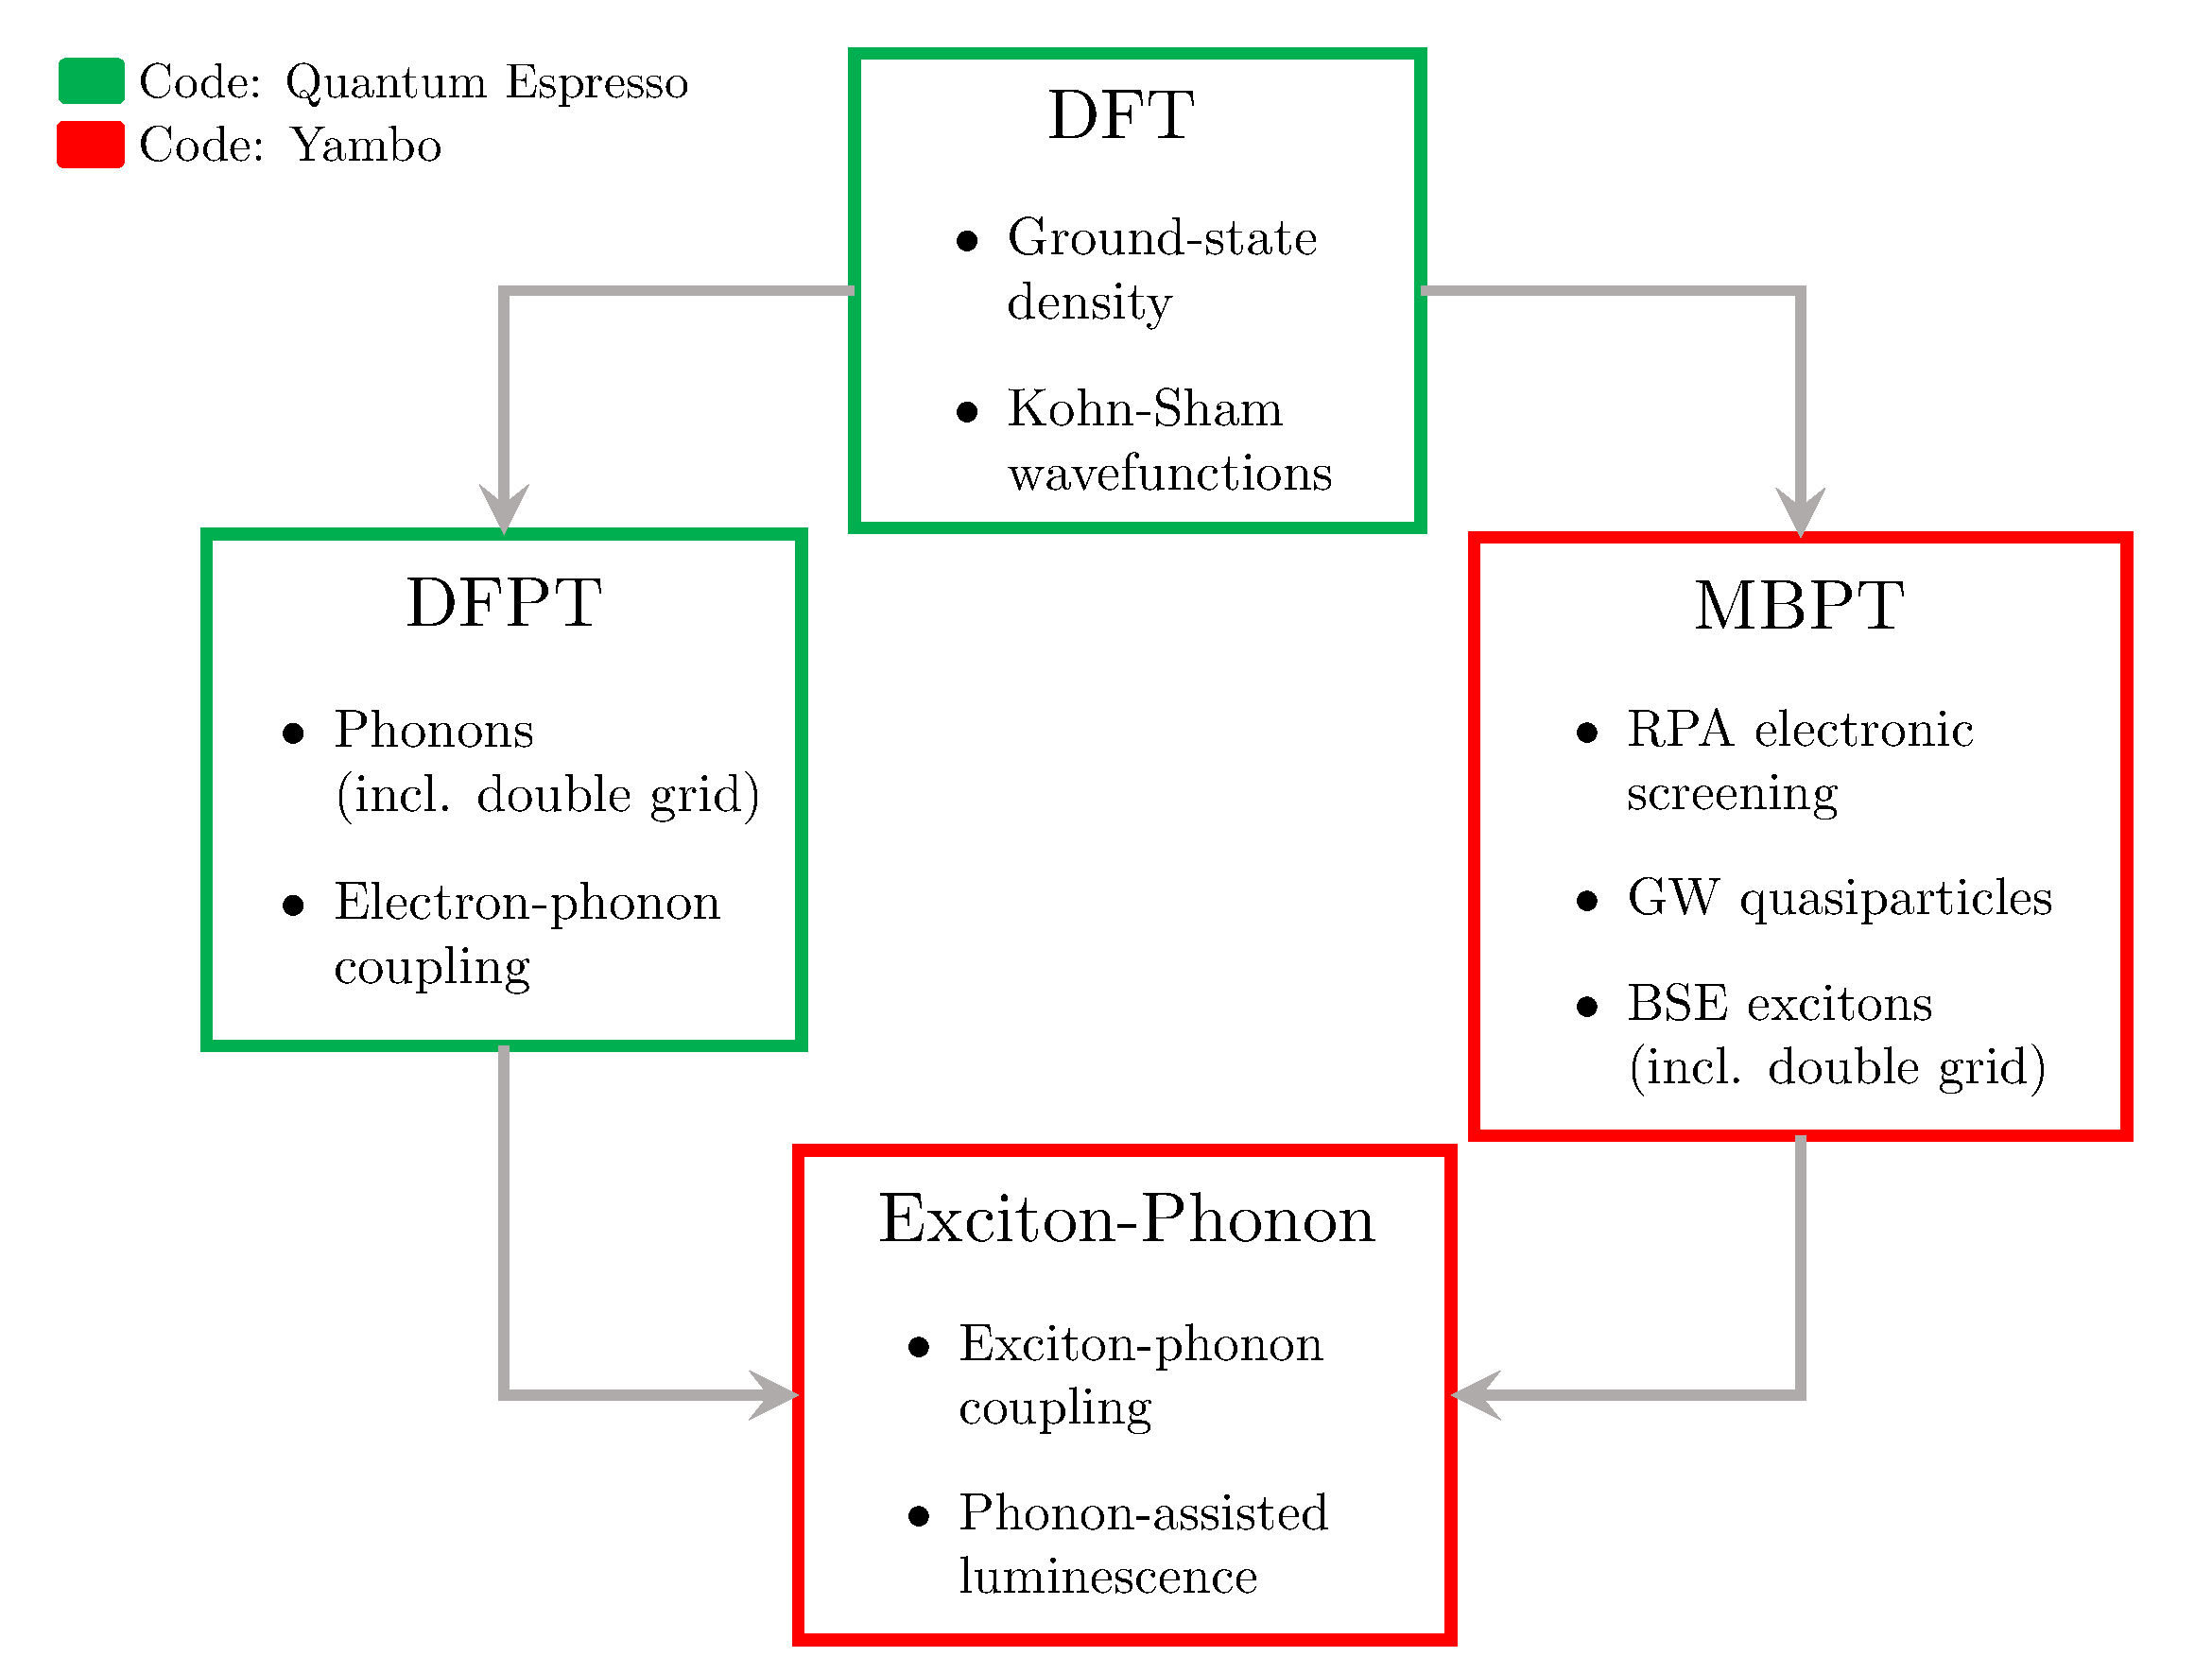
\includegraphics[width=0.9\textwidth]{intro/workflow_detailed.pdf}
	\caption{Workflow of the calculations to compute exciton-phonon coupling and phonon-assisted luminescence. The green and red boxes indicate that we used \textsc{Quantum ESPRESSO} and \yambo~as simulation codes, respectively.}
	\label{fig:workflow}
\end{figure}
The simulation code we used for \acrshort{DFT} and \acrshort{DFPT} is the \textsc{Quantum ESPRESSO} suite.\cite{giannozzi2009quantum,giannozzi2017advanced} For the \acrshort{MBPT} calculations, we used existing features of the \yambo~code,\cite{Sangalli_2019} and we implemented new features for the exciton-phonon coupling and phonon-assisted luminescence.

\section*{Structure}
This thesis is structured as follows. In Chapter \ref{chap:theory}, we summarize the theoretical background necessary to our exciton-phonon calculations and phonon-assisted luminescence. We start by briefly introducing \acrshort{DFT}, then we sketch a derivation of the Hedin's equations and obtain the \acrfull{GWA}. We proceed by deriving the \acrfull{BSE} and introducing the concept of \textit{excitons}. We present the link between the obtained many-body, microscopic quantities and the macroscopic observables measured in experiments. In the last part of this Chapter, we present \acrshort{DFPT}, the theory we use to compute \textit{phonons} and electron-phonon coupling from first-principles.

Chapter \ref{chap:strain} is devoted to bulk \acrshort{hBN} under strain. We present our results concerning the effect of uniaxial strain on the electronic, phononic and excitonic properties of \acrshort{hBN}. Then, we explain the finite-difference method we used to compute the exciton-phonon coupling in a static way, using displaced atoms in supercells. Finally, we show our luminescence results for the strained crystals and discuss their agreement with available experimental results.

In Chapter \ref{chap:mBN}, we present the derivation of the exciton-phonon coupling \textit{ab initio}, from first-order perturbation theory. From this we are able to obtain a response function containing a dynamical correction due to the coupling of excitons and phonons. We apply this approach to compute the luminescence spectrum of \acrfull{mBN} and address contradictory experimental interpretations of the structures therein. We also show preliminary results of the calculated luminescence of \acrfull{bBN}, which might exhibit both direct peak and phonon satellites with comparable intensities.
 
At the very end of this document, five appendices complement the main text and provide additional information on the materials and computational details.